\section{ErLam}

\subsection{The Language}

\begin{slide}
    \begin{figure}
    \centering
        {\footnotesize
            %%
%% ErLam BNF Style Grammar.
%%
\begin{BVerbatim}[commandchars=\\\{\}]
<Expression> ::= <Variable> 
              |  <Integer>
              |  `\textbf{newchan}'
              |  `\textbf{(}' <Expression> `\textbf{)}'
              |  <Expression> <Expression>
              |  `\textbf{if}' <Expression> <Expression> <Expression>
              |  `\textbf{swap}' <Channel> <Expression>
              |  `\textbf{spawn}' <Expression>
              |  `\textbf{fun}' <Variable> `\textbf{.}' <Expression>
\end{BVerbatim}

        }
    \label{fig:grammer}
    \end{figure}

    \inote{
        \item Extremely simple on purpose (5 keywords).
        \item Issue now began to be how to build up test primitives
        \item Made a library which allowed for built ins.
    }
\end{slide}

\begin{slide}
    \begin{figure}
    \centering
    \begin{BVerbatim}
elib
    // ...
    omega = (fun x.(x x));
    // ...
    add = _erl[2]{ fun(X) when is_integer(X) ->
                        fun(Y) when is_integer(Y) ->
                            X+Y
                        end
                    end
                 };
    // ...
bile
    \end{BVerbatim}
    \end{figure}

    \inote{
        \item Theres options for built-ins as well as macros.
    }
\end{slide}

\begin{SaveVerbatim}[commandchars=\\\{\}]{FibCode}
// pfib.els -
fun N.
    (omega \textbf{fun} f,m.(
        \textbf{if} (leq m 1) 
           m
           (merge \textbf{fun} _.(f f (sub m 1))
                  \textbf{fun} _.(f f (sub m 2))
                  add)) \textit{N})
\end{SaveVerbatim}

\begin{slide}
\framesubtitle{Example Application: Parallel Fibonacci}
    \begin{figure}
    \centering
    {\small
        \BUseVerbatim{FibCode}
    } 
    \end{figure}
    \begin{itemize}
        \item[] {\tt \$ els pfib.els}\hspace{8.65mm}(Compile the script)
        \item[] {\tt \$ ./pfib.ex -r 10}~~(Finds the 10th Fibonacci number)
    \end{itemize}
    
    \inote{
        \item R option is to run program applied to 10.
        \item To add more to this presentation than just reading paper
            I want to also give more detail as to system usage.
        \item Explain this Common Usage Pattern.
    }
\end{slide}

%%%%%%%%%%%%%%%%%%%%%%%%%%%%%%%%%%%%%%%%%%%%%%%%%%%%%%%%%%%%%%%%%%%%%%%%%%%%%%
\subsection{Channel Implementations}

\begin{slide}
    \begin{figure}
        \makebox[\textwidth][c]{
            \subfigure[t][Process Blocking Swap]{
                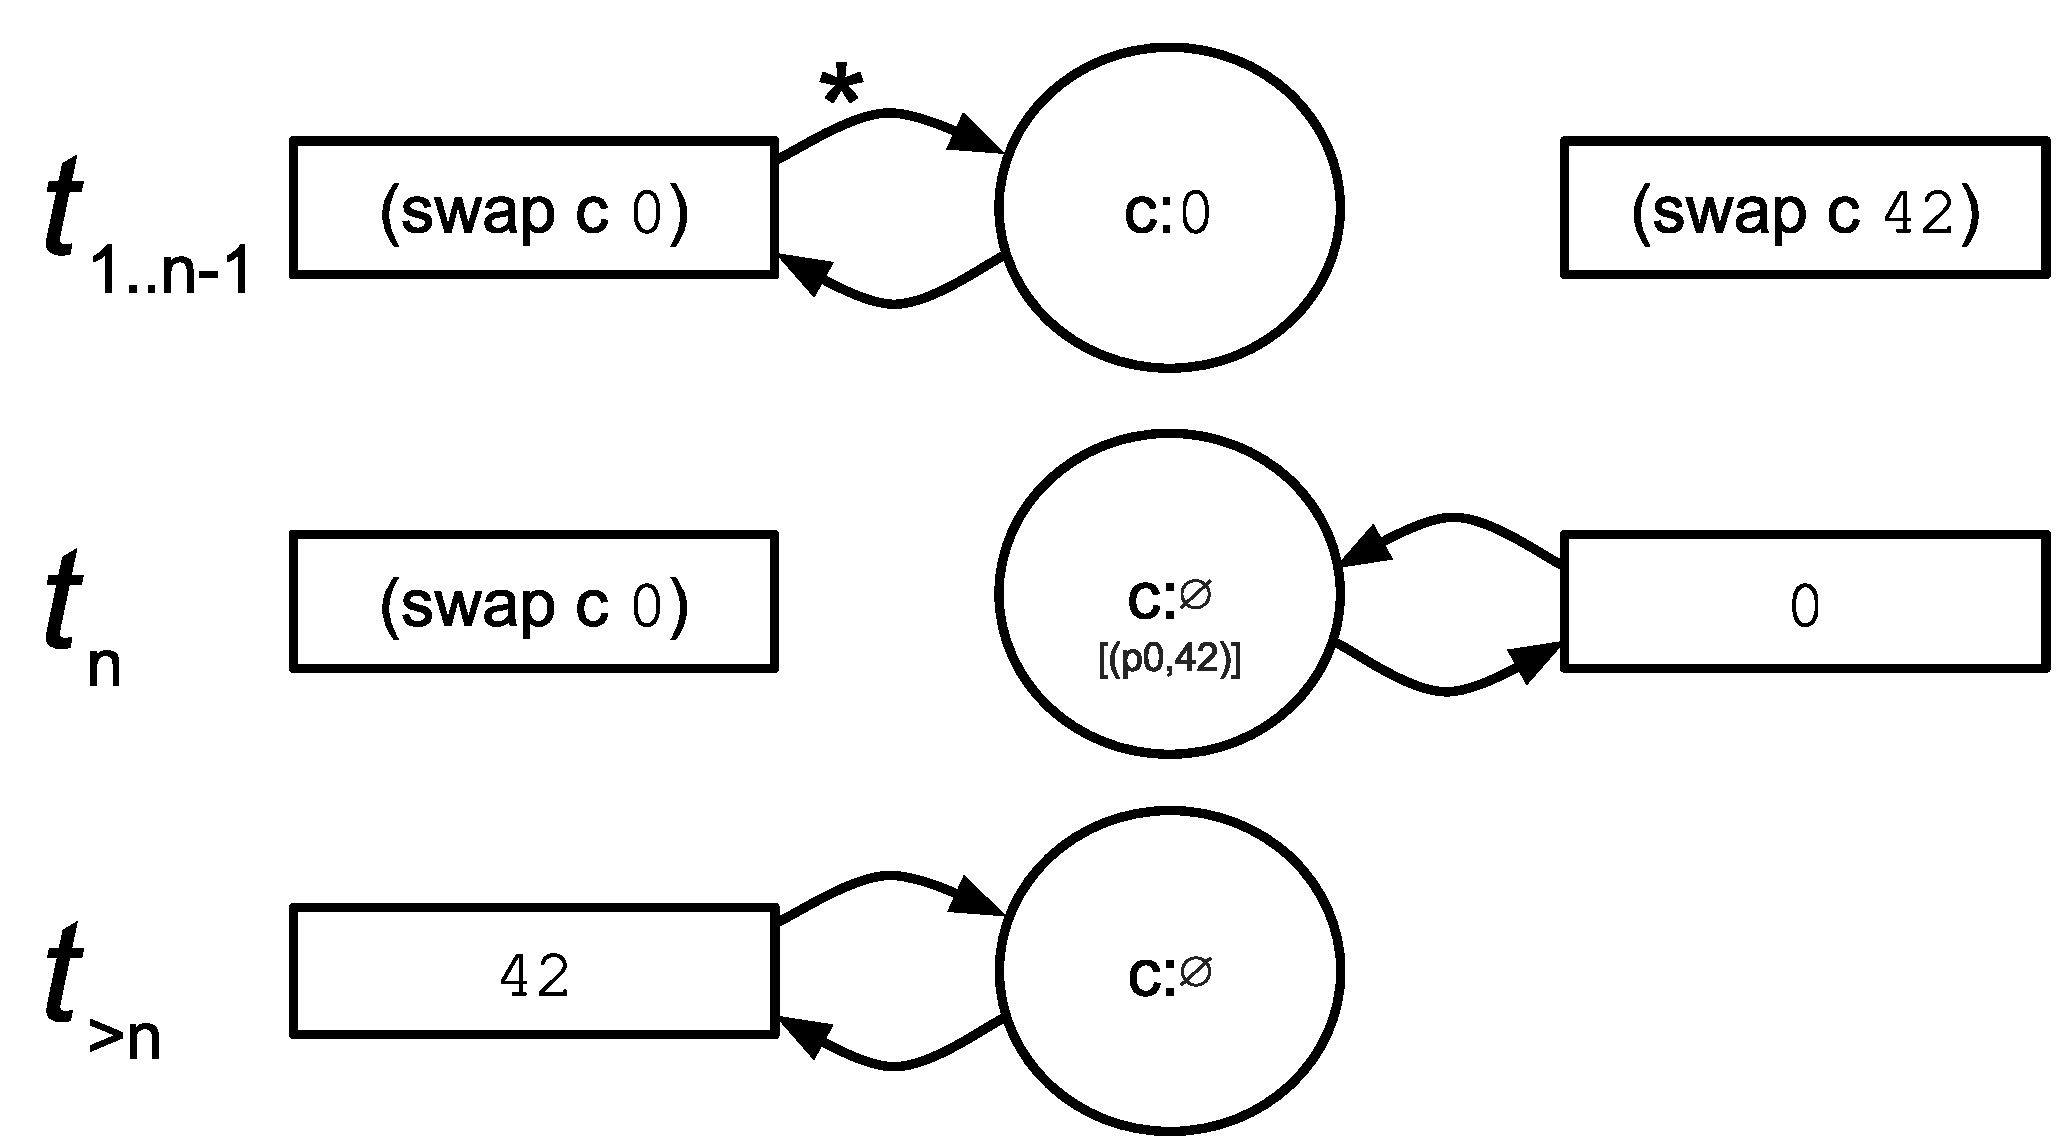
\includegraphics[width=0.5\textwidth]{BlockingSwap.pdf}
                \label{fig:blockchan-example}
            }  \subfigure[t][Process Absorption Swap]{
                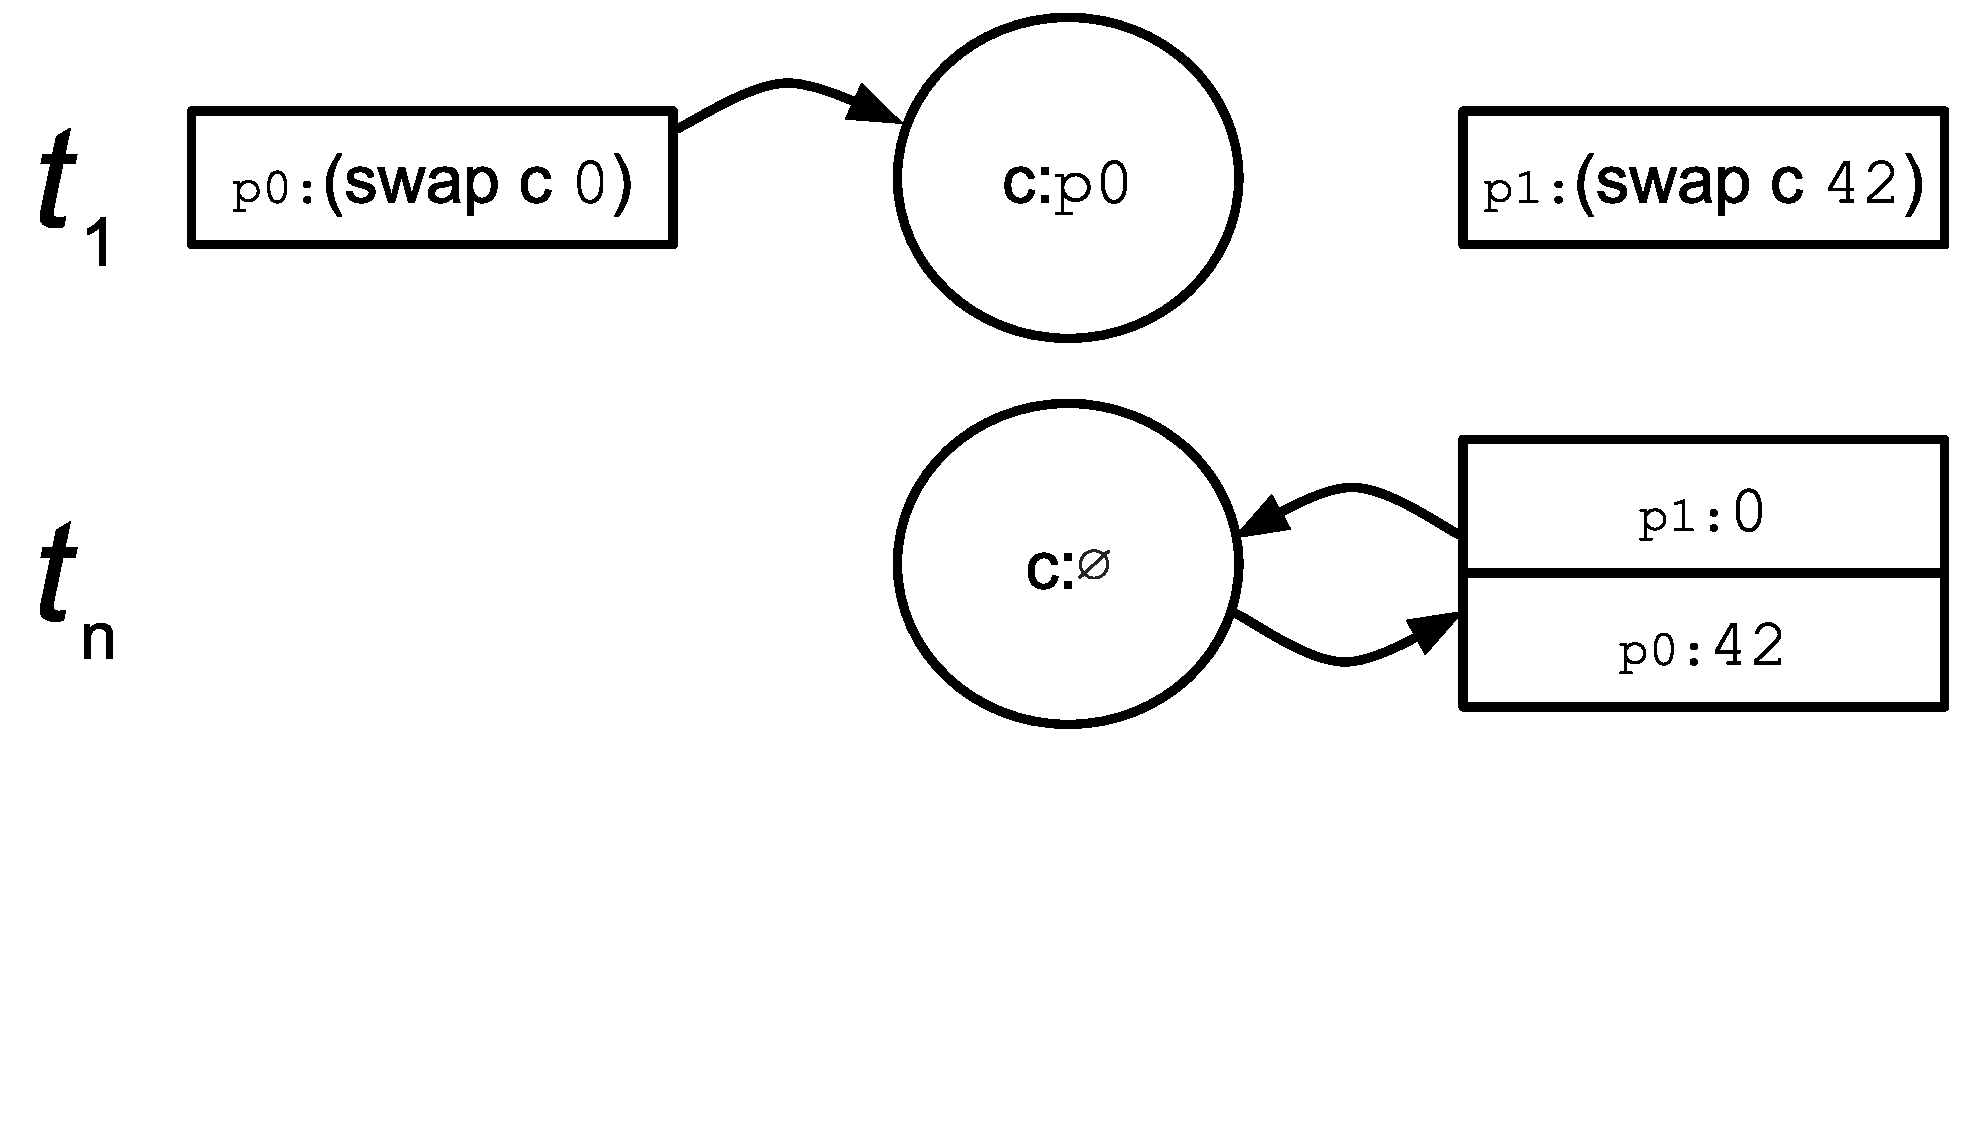
\includegraphics[width=0.5\textwidth]{AbsorbSwap2.pdf}
                \label{fig:absorbchan-example}
            }
        }
    \end{figure}
    \inote{
        \item Blocking: Maintains state of current and previous swap value until swap is completed.
        \item Absorption: Stores process which initializes the swap and returns it along with completion.
        \item Mention expected effects on scheduler.
        \item Blocking is default, passing '-a' to els 
    }
\end{slide}


%%%%%%%%%%%%%%%%%%%%%%%%%%%%%%%%%%%%%%%%%%%%%%%%%%%%%%%%%%%%%%%%%%%%%%%%%%%%%%
\subsection{Simulation \& Visualization}

\begin{slide}


    \inote{
        \item Need to talk about Chart types and chart generation.
    }
\end{slide}




















